\documentclass[11pt]{article}
\usepackage{fullpage}
\usepackage{amsmath, amsfonts}
\usepackage[utf8]{inputenc}
\usepackage{tikz}
\usepackage{graphicx}
\usepackage{booktabs}

\newcommand*{\Ph}{\hphantom{{}+{}}}%



\begin{document}
\begin{center}
{{\Large \sc Computational Discrete Mathematics}}
\end{center}
\rule{\textwidth}{1pt}
\begin{description}
\item[Student name and id:] Anders Launer Bæk (s160159)
%\item[Collaborator name(s) and id(s):] Morten Assive (s010101), Daniel Ata (s011001)
\item[Hand-in for week:] 4
\end{description}
\rule{\textwidth}{1pt}


\section*{Exercise 1}

Find the least period of the linear recurring sequence in $\mathbb{F}_{3}$ with eq. \ref{eq_1_1}.
\begin{equation}
\begin{align}
s_{n+4} = s_{n+3} + s_{n+2} - s_{n} -1, \quad n =0,1,..., \quad \in \quad  \mathbb{F}_{3}
\end{align}
\label{eq_1_1}
\end{equation}
where initial state vector is  $(0,-1,1,0)$.


%The corresponding characteristic polynomial is given in eq. \ref{eq_1_1_1}:
%\begin{equation}
%\begin{align}
%f(x) =x^4+x^3+x^2-x-1 \in \mathbb{F}_{3}[x]
%\end{align}
%\label{eq_1_1_1}
%\end{equation}

%and has the period of:
%\begin{equation}
%3^4-1 = 80
%\label{eq_1_1_2}
%\end{equation}

\begin{itemize}
\item Take the initial state vector  $(0,-1,1,0)$ and convert it to positive by taking $mod \quad 3$. It returns this initial state vector  $(0,2,1,0)$. Now apply eq. \ref{eq_1_1} for all $n$.
\begin{equation}
\begin{align}
%&= 0 \\
%&= -1 = 2\\
%&= 1\\
%&= 0 \\
s_{4} = s_{3} + s_{2} - s_{0} -1 &= 0 \\
s_{5} = s_{4} + s_{3} - s_{1} -1 &= 0 \\
s_{6} = s_{5} + s_{4} - s_{2} -1 &= 1 \\
s_{7} = s_{6} + s_{5} - s_{3} -1 &= 0 \\
& \vdots \\
s_{37} = s_{36} + s_{35} - s_{33} -1 &= 0 \\
s_{38} = s_{37} + s_{36} - s_{34} -1 &= 2 \\
s_{39} = s_{38} + s_{37} - s_{35} -1 &= 0 \\
s_{40} = s_{39} + s_{38} - s_{36} -1 &= 2 \\
s_{41} = s_{40} + s_{39} - s_{37} -1 &= 1 \\
s_{42} = s_{41} + s_{40} - s_{38} -1 &= 0 \\
s_{43} = s_{42} + s_{41} - s_{39} -1 &= ... \\
s_{44} = s_{43} + s_{42} - s_{40} -1 &= ...
\end{align}
\label{eq_1_2}
\end{equation}
\item The string of binary digits is from eq. \ref{eq_1_2}.
\begin{equation}
0	2	1	0|0	0	1	0	0	2	0	1	0	1	0	2	1	1	1	2	1	1	0	1	2	1	2	1	0	2	2	2	0	2	2	1	2	0	2	0	2	1	0	... ...		
\label{eq_1_3}
\end{equation}
The first four digits in eq. \ref{eq_1_3} are the initial state. 
\item The least period, from eq. \ref{eq_1_3},  is defined by when the initial state $(0,2,1,0)$ is represented in the sequence again. Eq. \ref{eq_1_4} states the least period.
\begin{equation}
LP = 39
\label{eq_1_4}
\end{equation}
\end{itemize}




















\newpage
\section*{Exercise 2}


A picture of the LFSR is given in figure \ref{fig_lfsr}.

\begin{figure}[th!]
\centering
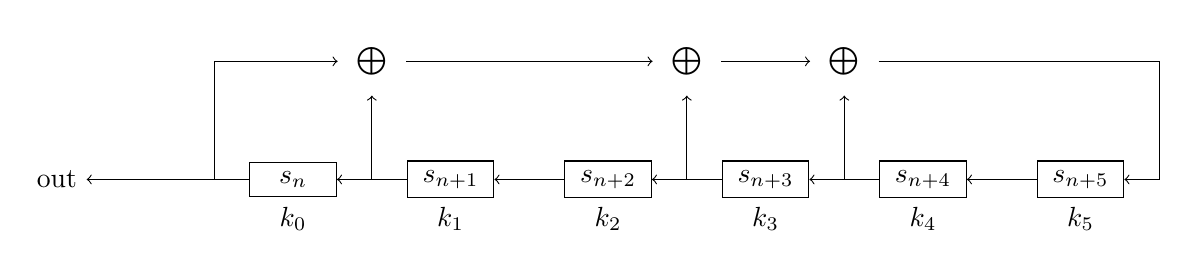
\begin{tikzpicture}

\node [] (out) at (-3,0) {out};

\node [draw=black, align=center, minimum width=1.1cm] (sn_0) at (0,0) {$s_n$};
\node [draw=black, align=center, minimum width=1.1cm] (sn_1) at (2,0) {$s_{n+1}$};
\node [draw=black, align=center, minimum width=1.1cm] (sn_2) at (4,0) {$s_{n+2}$};
\node [draw=black, align=center, minimum width=1.1cm] (sn_3) at (6,0) {$s_{n+3}$};
\node [draw=black, align=center, minimum width=1.1cm] (sn_4) at (8,0) {$s_{n+4}$};
\node [draw=black, align=center, minimum width=1.1cm] (sn_5) at (10,0) {$s_{n+5}$};


\node  (k_0) at (0,-0.5) {$k_0$};
\node  (k_0) at (2,-0.5) {$k_1$};
\node  (k_0) at (4,-0.5) {$k_2$};
\node  (k_0) at (6,-0.5) {$k_3$};
\node  (k_0) at (8,-0.5) {$k_4$};
\node  (k_0) at (10,-0.5) {$k_5$};




\node [circle, align=center] (add_1) at (1,1.5) {$\bigoplus$};
\node [circle, align=center] (add_2) at (5,1.5) {$\bigoplus$};
\node [circle, align=center] (add_3) at (7,1.5) {$\bigoplus$};

\draw[<-] (out)--(sn_0);
\draw[<-] (sn_0)--(sn_1);
\draw[<-] (sn_1)--(sn_2);
\draw[<-] (sn_2)--(sn_3);
\draw[<-] (sn_3)--(sn_4);
\draw[<-] (sn_4)--(sn_5);


\draw[<-] (add_1)--(1,0);
\draw[<-] (add_2)--(5,0);
\draw[<-] (add_3)--(7,0);

\draw[->] (add_1)--(add_2);
\draw[->] (add_2)--(add_3);
\draw[->] (add_3)--(11,1.5)--(11,0)--(sn_5);

\draw[<-] (add_1)--(-1,1.5)--(-1,0);


\end{tikzpicture}
\caption{LFSR from exercise 1-2 week 4.}
\label{fig_lfsr}
\end{figure}


Given the 10 bits of the key stream output as computed in exercise 2 and given in eq. \ref{eq_2_1}.
\begin{equation}
1|0111001101
\label{eq_2_1}
\end{equation}
The first bit from eq. \ref{eq_2_1} is from the "zero" state and the next ten are from the shifted states.

The filter function which we have to apply is given in eq. \ref{eq_2_2}. 

\begin{equation}
\phi(a,b,c,d) = ab \oplus bc \oplus ac \oplus d
\label{eq_2_2}
\end{equation}



From figure \ref{fig_lfsr} following eq. \ref{eq_2_30} must be true. 
\begin{equation}
k_5 = k_0  \oplus k_1  \oplus k_3  \oplus k_4
\label{eq_2_30}
\end{equation}

Write down at least 6 equations. See eq. \ref{eq_2_31} to eq. \ref{eq_2_36}
\begin{enumerate}
\item $\phi(s_0) = z_0$
\begin{equation}
\begin{align}
k_2k_3 \oplus k_3k_4 \oplus k_2k_4 \oplus k_5 &= 1 \quad mod \quad 2 \\
k_0 \oplus k_1 \oplus k_2 k_3 \oplus k_3 \oplus k_2 k_4 \oplus k_3 k_4 \oplus k_4 &=
\end{align}
\label{eq_2_31}
\end{equation}

\item $\phi(s_1) = z_1$
\begin{equation}
\begin{align}
k_1 \oplus k_2 \oplus k_3 k_4 \oplus k_4 \oplus k_3 k_5 \oplus k_4 k_5 \oplus k_5 &= 0 \quad mod \quad 2 \\
k_0k_3 \oplus k_1k_3 \oplus k_3^2 \oplus k_0k_4 \oplus k_1k_4 \oplus k_3k_4 \oplus k_4^2 \oplus k_0 \oplus k_2 \oplus k_3 &=
\end{align}
\label{eq_2_32}
\end{equation}

\item $\phi(s_2) = z_2$
\begin{equation}
\begin{align}
k_1k_2 \oplus k_2k_4 \oplus k_4^2 \oplus k_1k_5 \oplus k_2k_5 \oplus k_4k_5 \oplus k_5^2 \oplus k_1 \oplus k_3 \oplus k_4 &= 1 \quad mod \quad 2 \\
k_0^2 \oplus k_0k_1 \oplus k_0k_2 \oplus k_1k_3 \oplus k_2k_3 \oplus k_3^2 \oplus k_0k_4 \oplus k_3k_4 \oplus k_4^2 \oplus k_1 \oplus k_3 \oplus k_4&=
\end{align}
\label{eq_2_33}
\end{equation}



\item $\phi(s_3) = z_3$
\begin{equation}
\begin{align}
k_1^2 \oplus k_1k_2 \oplus k_1k_3 \oplus k_2k_4 \oplus k_3k_4 \oplus k_4^2 \oplus k_1k_5 \oplus k_4k_5 \oplus k_5^2 \oplus k_2 \oplus k_4 \oplus k_5&= 1 \quad mod \quad 2 \\
k_0^2 \oplus k_0k_1 \oplus k_1^2 \oplus k_1k_2 \oplus k_3^2 \oplus k_0k_4 \oplus k_2k_4 \oplus k_4^2 \oplus k_0 \oplus k_1 \oplus k_2 \oplus k_3&=
\end{align}
\label{eq_2_34}
\end{equation}



\item $\phi(s_4) = z_4$
\begin{equation}
\begin{align}
k_1^2 \oplus k_1k_2 \oplus k_1^2 \oplus k_2k_3 \oplus k_4^2 \oplus k_1k_5 \oplus k_2k_5 \oplus k_5^2 \oplus k_1 \oplus k_2 \oplus k_3 \oplus k_4 &= 1 \quad mod \quad 2 \\
k_0^2 \oplus k_0k_1 \oplus k_0k_2 \oplus k_1k_3 \oplus k_3^2 \oplus k_1k_4 \oplus k_2k_4 \oplus k_1 \oplus k_2 \oplus k_3 \oplus k_4&=
\end{align}
\label{eq_2_35}
\end{equation}



\item $\phi(s_5) = z_5$
\begin{equation}
\begin{align}
k_1^2 \oplus k_1k_2 \oplus k_1k_3 \oplus k_2k_4 \oplus k_4^2 \oplus k_2k_5 \oplus k_3k_5 \oplus k_2 \oplus k_3 \oplus k_4 \oplus k_5 &= 0 \quad mod \quad 2 \\
k_1^2 \oplus k_0k_2 \oplus k_0k_3 \oplus k_2k_3 \oplus k_3^2 \oplus k_3k_4 \oplus k_4^2 \oplus k_0 \oplus k_1 \oplus k_2&=
\end{align}
\label{eq_2_36}
\end{equation}
\end{enumerate}

%Eq. \ref{eq_2_31} to eq. \ref{eq_2_36} contains six equations with six unknown which is possible to solve.


\end{document}